\subsection{System simulations without controller}
To simulate the system (without control mechanism), we choose a series of numerical values, presented in table \ref{tab:numerical_values}\footnote{We would like to thank Professor Denoël for discussing these values with us.}.
\begin{table}[H]
    \centering
    \begin{tabular}{|l|c|c|}
        \hline
        {\bf Mass} & $m_1 = \SI{1e7}{\kilogram}$ & $m_2 = \SI{3e3}{\kilogram}$\\ \hline
        {\bf Spring} & $k_1 \approx \SI{4e8}{\newton/\meter}$ & $k_2 = \SI{e5}{\newton/\meter}$\\ \hline
        {\bf Damper} & $c_1 \approx \SI{1.3e6}{\newton\second/\meter}$ & $c_2 = \SI{e4}{\newton\second/\meter}$\\ \hline
        {\bf Wind} & \multicolumn{2}{c|}{$F_{max} = \SI{810000}{\newton}$}\\ \hline
    \end{tabular}
    \caption{Numerical values of the system}
    \label{tab:numerical_values}
\end{table}
For the strength of the wind, we considered 2 cases (in newton) :
\begin{align*}
    F_1 &= F_{max}\quad\forall t & \text{Constant wind force}\\
    F_1(t) &= F_{max}\sin(2\pi t) & \text{Sinusoidal wind force}
\end{align*}
The stiffness and viscosity values for the building were obtained using the formulas :
\begin{align*}
    k_1 &= (2\pi f)^2m_1\\
    c_1 &= 2m_1(2\pi f)0.01
\end{align*}
where $f = \SI{1}{\hertz}$ is the natural frequency associated with the mass of the building.\par
The maximum wind force, on the other hand, was approximated by
\begin{equation*}
    F_{max} = \frac{1}{2}\rho v^2A
\end{equation*}
with
\begin{itemize}
    \item $\rho \approx \SI{1.2}{\kilogram/\meter\cubed}$, the air density;
    \item $v = \SI{15}{\meter/\second}$, the wind speed;
    \item $A = 200\times 30 = \SI{6000}{\meter\squared}$, the area of one side of the building.
\end{itemize}
\subsubsection{Simulation results}
\begin{figure}[H]
    \centering
    \begin{subfigure}{0.495\textwidth}
        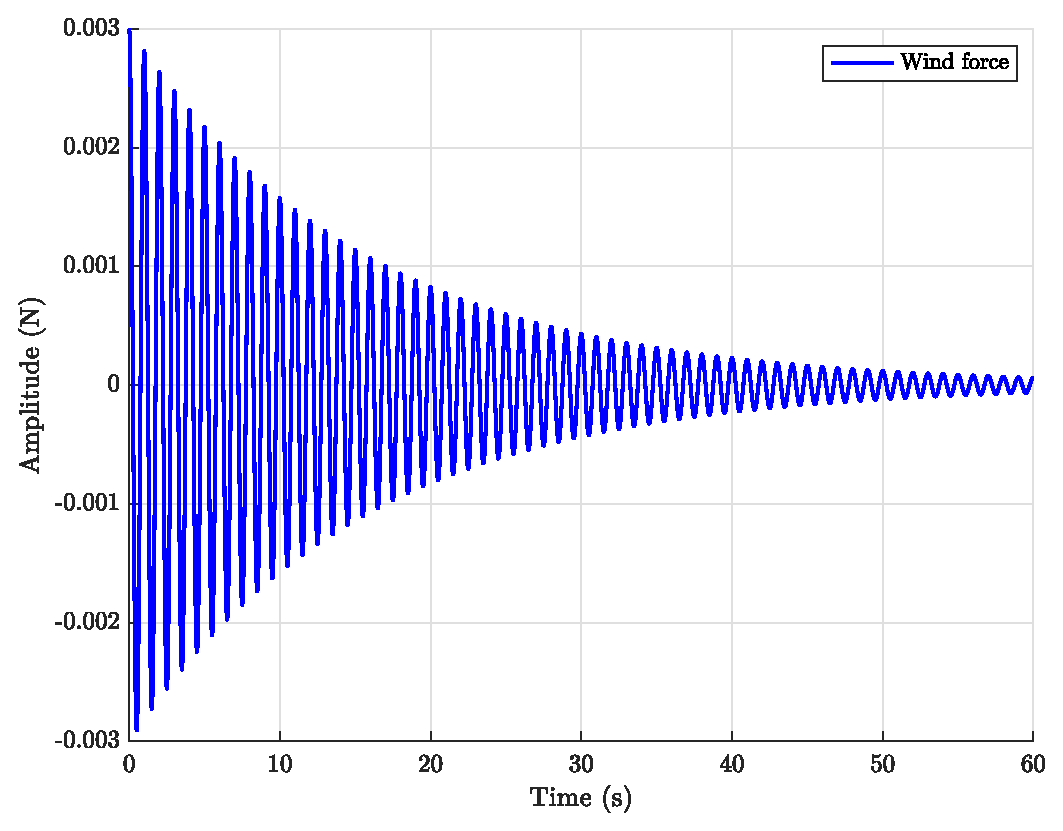
\includegraphics[width=\textwidth]{resources/eps/initial-condition.eps}
        \caption{Initial conditions}
        \label{fig:q4.initial}
    \end{subfigure}
    \begin{subfigure}{0.495\textwidth}
        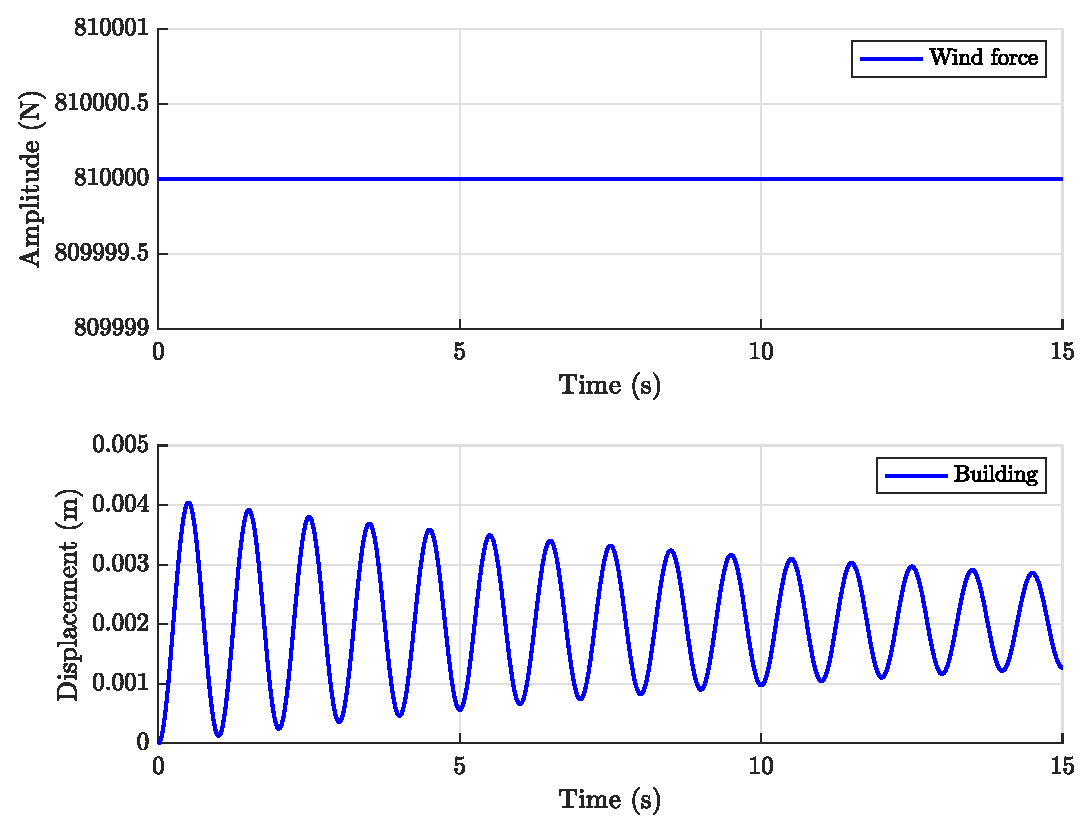
\includegraphics[width=\textwidth]{resources/eps/constant-wind.eps}
        \caption{Constant wind force}
        \label{fig:q4.constant}
    \end{subfigure}
    \begin{subfigure}{0.495\textwidth}
        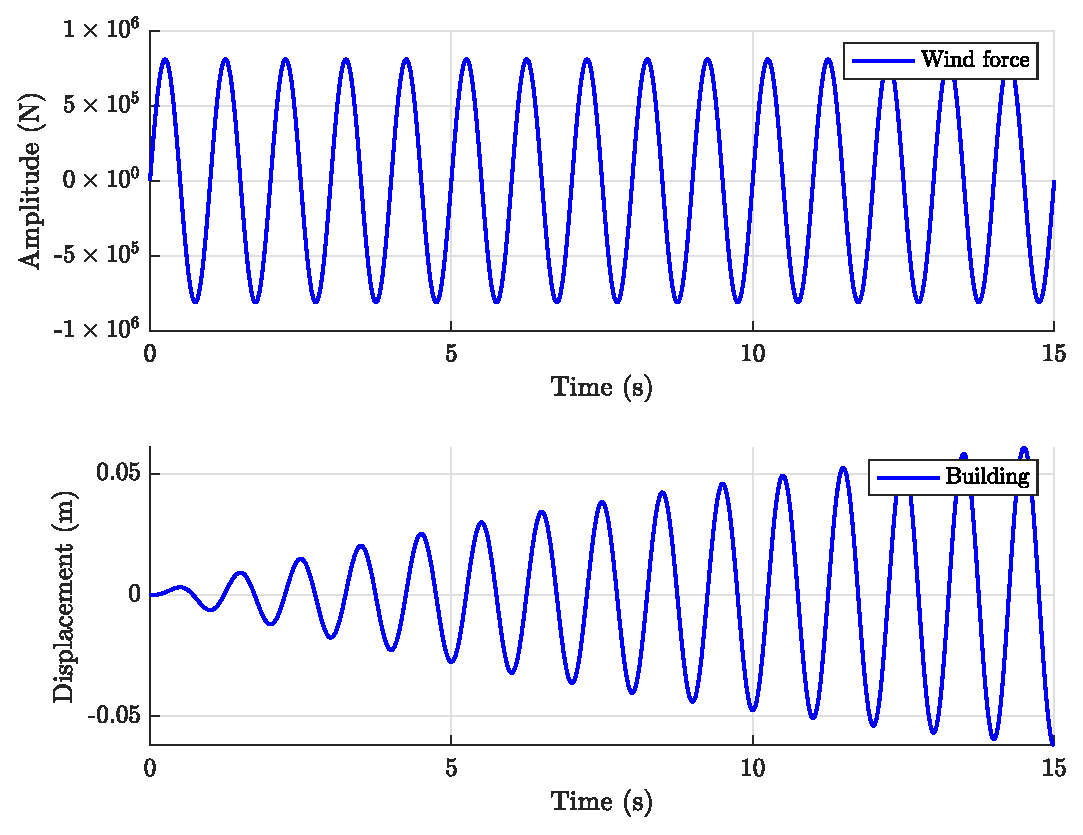
\includegraphics[width=\textwidth]{resources/eps/sinusoidal-wind.eps}
        \caption{Sinusoidal wind force}
    \end{subfigure}
    \begin{subfigure}{0.495\textwidth}
        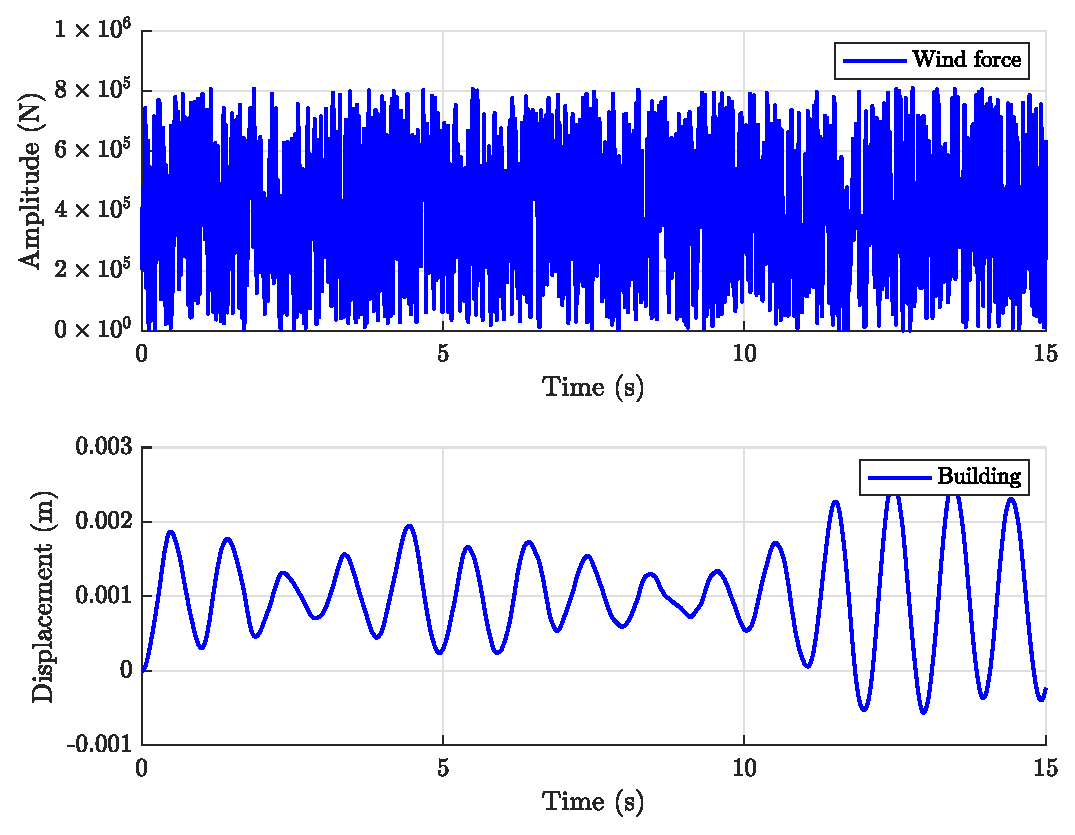
\includegraphics[width=\textwidth]{resources/eps/random-wind.eps}
        \caption{Random wind force}
    \end{subfigure}
    \noskipcaption{Simulation results}
\end{figure}
The first simulation (figure \ref{fig:q4.initial}) is a response of our system to initial conditions : the initial displacement of the building is defined at \SI{0.5}{\meter}. We observe that the building oscillates and tends to regain its reference position.\par
The other simulations are responses of our system to an input (the wind).\par
In the case of a constant force (figure \ref{fig:q4.constant}), the building oscillates at the beginning and then tends to stabilize (at a position different from its reference).\par
In cases of sinusoidal and random forces, the building oscillates and follows approximately the wind movement.
